% ============================================================
%  FINDEC-RS — Project Proposal (Midterm)
%  Behavioral Bias-Aware Personalized Investment Recommender
%  System using Multi-Agent Profiling and Knowledge Graphs
% ============================================================
\documentclass[12pt, a4paper]{article}

% ── Packages ────────────────────────────────────────────────
\usepackage[T1]{fontenc}
\usepackage[utf8]{inputenc}
\usepackage{lmodern}
\usepackage[margin=2.2cm, top=2.8cm, bottom=2.8cm]{geometry}
\usepackage{graphicx}
\usepackage{xcolor}
\usepackage{amsmath, amssymb}
\usepackage{booktabs}
\usepackage{tabularx}
\usepackage{array}
\usepackage{longtable}
\usepackage{multirow}
\usepackage{enumitem}
\usepackage{hyperref}
\usepackage{fancyhdr}
\usepackage{titlesec}
\usepackage{tocloft}
\usepackage{caption}
\usepackage{float}
\usepackage{tikz}
\usepackage{pgf-pie}
\usepackage{mdframed}
\usepackage{setspace}
\usepackage{microtype}
\usepackage{cite}
\usepackage{url}
\usepackage[most]{tcolorbox}
\usepackage{fontawesome5}
\usepackage{parskip}
\usepackage{afterpage}

\usetikzlibrary{shapes.geometric, arrows.meta, positioning, fit,
                backgrounds, shadows.blur, calc, decorations.pathreplacing}

% ── Colours ─────────────────────────────────────────────────
\definecolor{darkblue}{HTML}{000000}
\definecolor{midblue}{HTML}{1A1A1A}
\definecolor{accentblue}{HTML}{333333}
\definecolor{lightbg}{HTML}{F5F5F5}
\definecolor{verylightbg}{HTML}{FAFAFA}
\definecolor{greytext}{HTML}{555555}
\definecolor{lightgrey}{HTML}{EEEEEE}
\definecolor{successgreen}{HTML}{000000}
\definecolor{successbg}{HTML}{F0F0F0}
\definecolor{agentred}{HTML}{000000}
\definecolor{agentpurple}{HTML}{1A1A1A}
\definecolor{agentteal}{HTML}{333333}

% ── Hyperref setup ──────────────────────────────────────────
\hypersetup{
    colorlinks   = true,
    linkcolor    = black,
    citecolor    = black,
    urlcolor     = black,
    pdftitle     = {FINDEC-RS Project Proposal},
    pdfauthor    = {Mansi},
    pdfsubject   = {Recommender Systems Midterm Proposal},
}

% ── Section title formatting ────────────────────────────────
\titleformat{\section}
  {\Large\bfseries\color{black}}
  {\thesection}{0.8em}{}
  [\vspace{6pt}\hrule\vspace{4pt}]

\titleformat{\subsection}
  {\large\bfseries\color{black}}
  {\thesubsection}{0.6em}{}
  [\vspace{2pt}]

\titleformat{\subsubsection}
  {\normalsize\bfseries\color{black}}
  {\thesubsubsection}{0.5em}{}
  [\vspace{1pt}]

% ── Header / Footer ─────────────────────────────────────────
\pagestyle{fancy}
\fancyhf{}
\fancyhead[L]{\small\textbf{FINDEC-RS} \, | \, \textcolor{greytext}{Behavioral Bias-Aware Investment Recommender System}}
\fancyhead[R]{\small\textcolor{greytext}{Midterm Proposal}}
\fancyfoot[C]{\small\textcolor{greytext}{\thepage}}
\fancyfoot[L]{\small\textcolor{greytext}{Department of Computer Science}}
\fancyfoot[R]{\small\textcolor{greytext}{Recommender Systems Course}}
\renewcommand{\headrulewidth}{0.5pt}
\renewcommand{\footrulewidth}{0.5pt}
\renewcommand{\headrule}{\color{black}\hrule width\headwidth height\headrulewidth \vskip-\headrulewidth}

% ── TOC formatting ──────────────────────────────────────────
\renewcommand{\cftsecfont}{\bfseries\color{black}}
\renewcommand{\cftsubsecfont}{\color{black}}
\renewcommand{\cftsecpagefont}{\bfseries\color{black}}
\setlength{\cftbeforesecskip}{6pt}

% ── Custom box environments ─────────────────────────────────
\tcbset{
  gapbox/.style={
    enhanced, breakable,
    colback=verylightbg, colframe=black,
    boxrule=1.2pt, arc=3pt,
    left=10pt, right=10pt, top=8pt, bottom=8pt,
    fonttitle=\bfseries\color{black},
    title style={fill=lightbg, draw=black, line width=0.5pt},
  },
  objbox/.style={
    enhanced, breakable,
    colback=verylightbg, colframe=black,
    boxrule=1pt, arc=3pt,
    left=10pt, right=10pt, top=8pt, bottom=8pt,
    fonttitle=\bfseries\small\color{black},
  },
  abstractbox/.style={
    enhanced,
    colback=lightbg, colframe=black,
    boxrule=1.5pt, arc=4pt,
    left=12pt, right=12pt, top=10pt, bottom=10pt,
  }
}

% ── Spacing ─────────────────────────────────────────────────
\onehalfspacing
\setlength{\parskip}{6pt}
\setlength{\parindent}{0pt}
\setlist[itemize]{noitemsep, topsep=4pt, leftmargin=1.8cm}
\setlist[enumerate]{noitemsep, topsep=4pt, leftmargin=1.8cm}

% ============================================================
\begin{document}

% ── Title Page ──────────────────────────────────────────────
\begin{titlepage}
\pagecolor{black}
\centering
\color{white}

% Title
\vspace*{1.5cm}
{\Huge\bfseries FINDEC-RS}
\vspace{0.7cm}

% Subtitle
{\Large
Behavioral Bias-Aware Personalized Investment\\
Recommender System using Multi-Agent\\
Profiling and Knowledge Graphs}
\vspace{0.9cm}

% Decorative line
{\color{white}\rule{10cm}{0.5pt}}
\vspace{0.9cm}

% Project details
{\large \textit{Midterm Project Proposal}}\\[10pt]
{\normalsize Recommender Systems --- Spring 2025}

\vspace{1.8cm}

% Submission box
\begin{tcolorbox}[
  enhanced, width=10.5cm,
  colback=white, colframe=white,
  boxrule=0pt, arc=2pt,
  center,
  fontupper=\color{black}
]
  \centering
  {\bfseries\large Submitted by}\\[10pt]
  {\Huge Mansi}\\[10pt]
  {SID: 22103045}\\[8pt]
  {Submitted to: Ms. Shilpa Verma}\\[6pt]
  {Session: 2022-2026}
\end{tcolorbox}

\vspace{2cm}

% Implementation details
{\small\color{white}
  \textbf{Implementation Language:} Python 3.11 \quad | \quad
  \textbf{Platform:} Web (Next.js 14 + FastAPI)
}

\vfill

% Footer
{\color{white}\rule{10cm}{0.5pt}}\\[10pt]
{\small\color{white} Department of Computer Science --- Recommender Systems --- 2025}

\end{titlepage}

\newpage
\pagecolor{white}
\color{black}

% ============================================================
\section{Project Proposal}

% ── 1.1 ─────────────────────────────────────────────────────
\subsection{Title and Abstract}

\textbf{Title:}\\
\textit{FINDEC-RS: Behavioral Bias-Aware Personalized Investment Recommender System
using Multi-Agent Profiling and Knowledge Graphs}

\vspace{0.5cm}
\textbf{Abstract}

\begin{tcolorbox}[abstractbox]
Modern retail investors face two compounding challenges that existing platforms entirely
ignore. First, investors routinely make \textbf{irrational financial decisions} driven by
well-documented cognitive biases --- loss aversion, overconfidence, recency bias, and
herding behaviour --- causing systematic deviation from optimal portfolio outcomes.
Second, \textbf{investment intent is inherently multi-dimensional}: a single investor
simultaneously weighs expected returns, tolerable risk, industry sector preferences, and
trust in specific fund managers, yet existing platforms collapse this high-dimensional
intent into a single scalar risk label, producing misaligned recommendations.

FINDEC-RS addresses both challenges through a three-agent AI pipeline tightly coupled
with a dynamic Knowledge Graph (KG)-based Recommender System. The \textit{Bias Detector
Agent} analyses behavioural interaction signals to classify each user's dominant bias
profile. The \textit{Multi-Factor Intent Modeler} constructs a structured intent vector
encoding return expectations, risk appetite, sector affinities, and fund-manager trust
scores. The \textit{Recommender Agent} fuses these signals over a dynamic KG and applies
Graph Neural Network (GNN)-based collaborative filtering to generate personalised,
bias-corrected, explainable asset rankings. The system is delivered as a full-stack web
application (Next.js 14 + FastAPI) evaluated on Precision@K, Recall@K, NDCG, Novelty,
Diversity, and simulated financial performance metrics.
\end{tcolorbox}

% ── 1.2 ─────────────────────────────────────────────────────
\subsection{Keywords}

\begin{center}
\textbf{
Recommender Systems \quad $\cdot$ \quad Behavioral Finance \quad $\cdot$ \quad
Cognitive Bias Debiasing \quad $\cdot$ \quad Knowledge Graphs \\[6pt]
Graph Neural Networks \quad $\cdot$ \quad Multi-Agent Systems \quad $\cdot$ \quad
Investment Personalization \\[6pt]
Multi-Factor Intent Modeling \quad $\cdot$ \quad Explainable AI \quad $\cdot$ \quad
FinTech Recommender Systems
}
\end{center}

% ── 1.3 ─────────────────────────────────────────────────────
\subsection{Introduction}

The rapid democratisation of retail investing through platforms such as Zerodha, Robinhood,
Groww, and Tickertape has lowered barriers to market participation; yet a critical
personalisation gap persists. These platforms surface identical screened assets to all
users sharing a broad risk category, entirely disregarding how individual psychology shapes
investment behaviour and how multifaceted a single user's intent truly is.

\subsubsection*{Challenge 1 --- Irrational Investor Behaviour}

Behavioural finance research has rigorously documented that investors deviate
\textit{systematically} from rationality in structured, predictable ways. \textit{Loss aversion}
causes disproportionate reactions to losses relative to equivalent gains. \textit{Overconfidence}
leads to excessive trading and under-diversification. \textit{Recency bias} skews portfolios
toward recent winners. \textit{Herding} drives investors to follow crowd sentiment rather than
fundamentals. Crucially, these biases are not random noise --- they are user-specific, persistent,
and predictable, yet no existing Recommender System (RS) exploits this structure to \textit{correct}
recommendations rather than reinforce them.

\subsubsection*{Challenge 2 --- Multi-Dimensional Investment Intent}

When an investor evaluates a mutual fund or equity, the decision integrates multiple
simultaneous factors: anticipated return over a target horizon, acceptable volatility or
drawdown, alignment with preferred sectors (e.g., renewable energy, technology), and ---
critically in the retail investment context --- trust in the fund manager's historical
track record and reputation. Current RS models collapse this high-dimensional intent into
a single scalar (star rating or risk score), causing misaligned recommendations and eroding
user trust.

\subsubsection*{Proposed Solution Summary}

FINDEC-RS proposes a unified three-agent pipeline where each agent serves a
non-redundant role: bias profiling, intent vector construction, and KG-augmented GNN
recommendation. The system directly addresses both challenges and produces
explainable, behaviorally-grounded recommendations that tell the user not just
\textit{what} to consider but \textit{why} --- including which of their own biases
the recommendation is designed to correct.

% ── 1.4 ─────────────────────────────────────────────────────
\subsection{Objectives}

\begin{tcolorbox}[objbox, title={Objective 1 --- Behavioral Bias Detection and Profiling}]
Design and implement a \textbf{Bias Detector Agent} capable of inferring dominant
cognitive biases (loss aversion, overconfidence, recency bias, herding) from implicit
user interaction signals --- trade frequency, hold duration, watchlist churn, query
patterns --- with classification accuracy exceeding 80\%. This agent will produce a
per-user \textit{bias profile vector} with confidence scores across four bias dimensions,
updated at each session.
\end{tcolorbox}

\begin{tcolorbox}[objbox, title={Objective 2 --- Multi-Factor Intent Representation}]
Develop a \textbf{Multi-Factor Intent Modeler} that constructs a structured intent vector
$\mathbf{i}_u = [\alpha_{\text{return}},\ \alpha_{\text{risk}},\ \vec{\alpha}_{\text{sector}},\ \vec{\alpha}_{\text{fund\_mgr}}]$ per user, combining explicit onboarding signals and implicit
behavioural inference (assets viewed, time spent, filters applied). This vector is updated
continuously and stored as a dynamic node attribute in the Knowledge Graph, enabling
temporal intent tracking across sessions.
\end{tcolorbox}

\begin{tcolorbox}[objbox, title={Objective 3 --- Knowledge Graph-Augmented Recommendation}]
Build a dynamic Knowledge Graph connecting users, assets, sectors, bias types, and intent
dimensions, and train a \textbf{Graph Neural Network} (GraphSAGE or GAT) over this KG to
generate bias-corrected, intent-aligned, personalised asset rankings. Performance to be
measured by NDCG, Precision@K, Novelty, and Diversity against collaborative filtering
baselines.
\end{tcolorbox}

\begin{tcolorbox}[objbox, title={Objective 4 --- Explainable Web Interface}]
Deliver a full-stack web application (Next.js 14 + FastAPI) where users receive
\textbf{natural-language explanations} for each recommendation --- specifying which intent
dimensions were satisfied and which biases the recommendation mitigates. The interface
will include a live bias-profile dashboard, recommendation feed with KG-traced explanation
chips, and a portfolio overview panel.
\end{tcolorbox}

% ── 1.5 ─────────────────────────────────────────────────────
\subsection{Research Gaps}

\begin{tcolorbox}[gapbox, title={\faSearch\ Gap 1 --- Behavioral Biases Absent from RS Pipelines}]
Despite decades of behavioural finance literature confirming that cognitive biases
systematically distort investment decisions, no existing financial RS incorporates bias
detection as a first-class input to the recommendation ranking function. Platforms such
as Tickertape apply identical logic to all users within a risk tier, ignoring that two
``medium-risk'' users may exhibit diametrically opposite bias profiles. The RS thereby
\textit{actively reinforces} suboptimal behaviour rather than correcting it.
\end{tcolorbox}

\begin{tcolorbox}[gapbox, title={\faDatabase\ Gap 2 --- Collapse of Multi-Dimensional Investment Intent}]
Existing financial RS reduce user preferences to a unidimensional risk score or broad
category label (conservative / balanced / aggressive). This abstraction discards crucial
orthogonal preference axes: expected returns, sector alignment, and fund manager trust
operate \textit{independently}, yet no current RS formalises these as a structured,
learnable intent vector. Recent intent-modeling research confirms that incorporating
real-time intent prediction yields measurable improvements, but such work is limited to
entertainment platforms and has not been applied to the structured multi-factor intent
space of investment decision-making.
\end{tcolorbox}

\begin{tcolorbox}[gapbox, title={\faSitemap\ Gap 3 --- Static Knowledge Graphs in Financial RS}]
The limited literature on KG-based financial RS constructs \textit{static} graphs
capturing asset--sector--attribute relationships at a fixed point in time. User cognitive
state, bias evolution, and changing intent are never modelled as KG nodes or edges.
FINDEC-RS introduces \textbf{dynamic user-state nodes} updated at each interaction session,
enabling the GNN to reason over a living representation of the investor --- an approach
absent from the KG-RS literature.
\end{tcolorbox}

\begin{tcolorbox}[gapbox, title={\faComments\ Gap 4 --- Absence of Behaviorally-Grounded Explainability}]
When financial platforms do offer explanations, they cite generic factors
(``matches your risk profile''). No system provides explanations that reference the user's
own detected biases. While recent multi-agent RS frameworks improve contextual reasoning,
\textit{behaviorally-grounded} explainability that directly maps detected cognitive bias
to recommendation rationale remains entirely unaddressed.
\end{tcolorbox}

% ── 1.6 ─────────────────────────────────────────────────────
\subsection{Proposed Solution}

FINDEC-RS is structured around three tightly coupled components: a Multi-Agent Pipeline,
a dynamic Knowledge Graph, and a GNN-based Recommender Engine, all surfaced through a
full-stack web interface.

\subsubsection{System Architecture}

The FINDEC-RS system architecture consists of three main layers:

\begin{enumerate}[leftmargin=1.5cm]
  \item \textbf{Multi-Agent Pipeline Layer:}
  \begin{itemize}
    \item Bias Detector Agent: Classifies user cognitive biases from interaction signals
    \item Intent Modeler Agent: Constructs multi-factor intent vectors
    \item Recommender Agent: Generates personalized recommendations
  \end{itemize}
  
  \item \textbf{Knowledge Graph Layer:}
  \begin{itemize}
    \item Dynamic graph with user, asset, bias, intent, sector, and fund manager nodes
    \item Real-time updates as user behavior patterns emerge
    \item Semantic relationships capturing bias corrections and intent alignments
  \end{itemize}
  
  \item \textbf{Inference Layer:}
  \begin{itemize}
    \item Graph Neural Network encoder (GraphSAGE or GAT)
    \item Bias-correction weighting mechanism
    \item Natural language explanation generator
  \end{itemize}
\end{enumerate}

\begin{figure}[H]
\centering
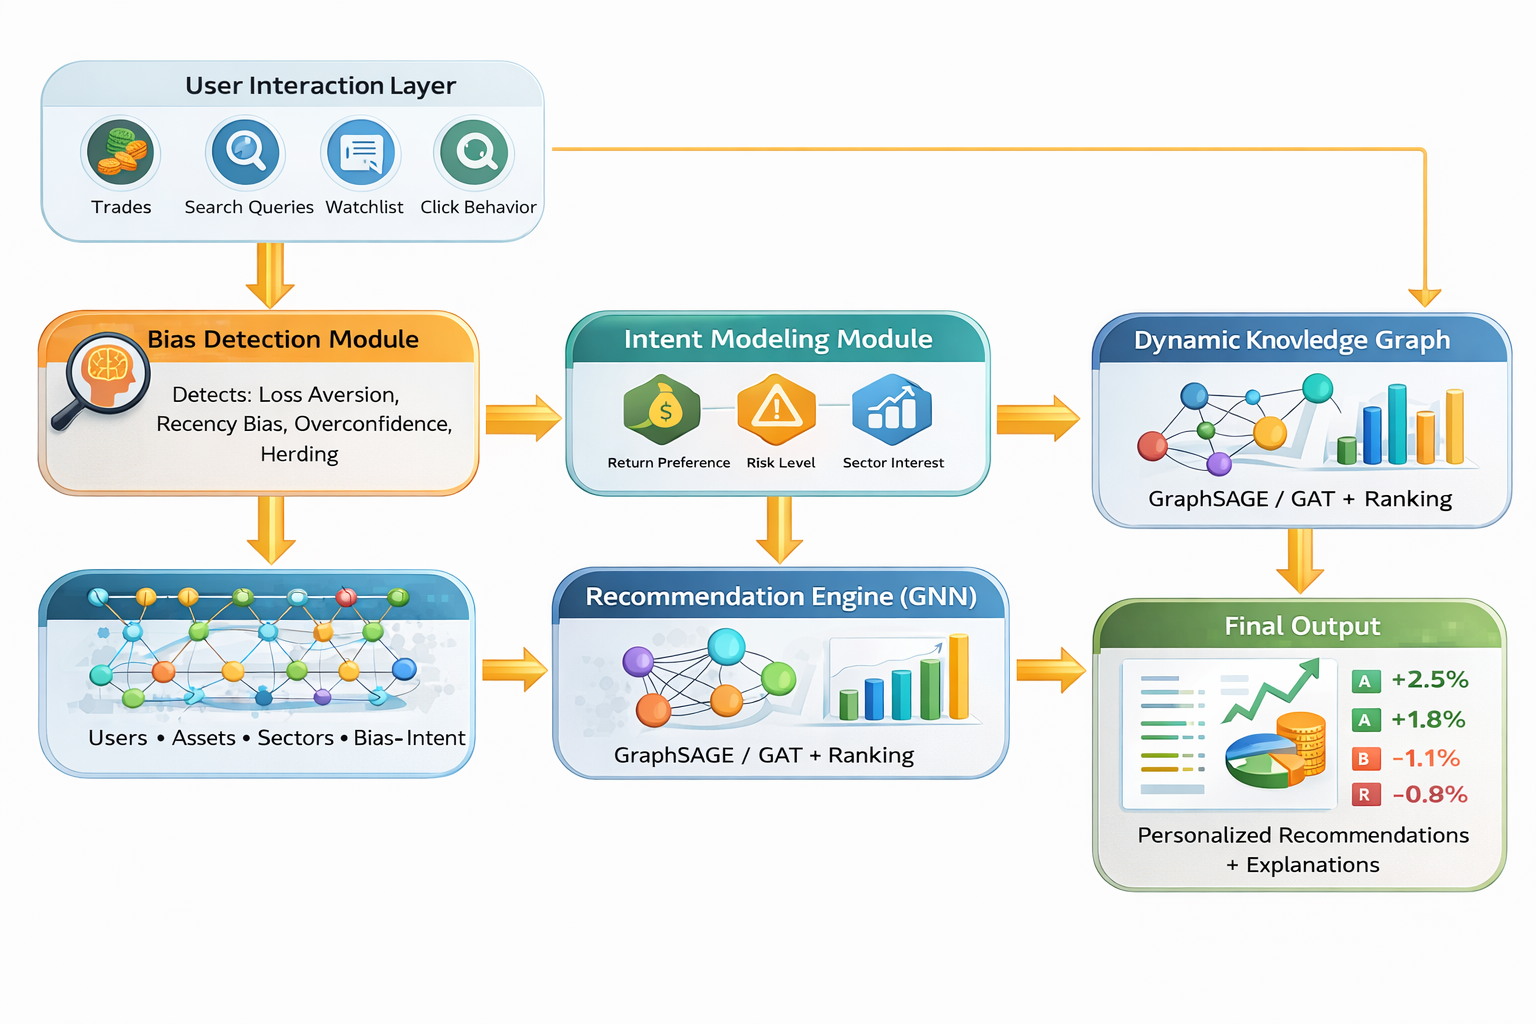
\includegraphics[width=0.95\textwidth]{figures/system_design_architecture.png}
\caption{FINDEC-RS System Architecture. The pipeline processes user interaction data through 
multi-agent profiling (Bias Detector, Intent Modeler, and Recommender agents), dynamic knowledge 
graph construction, and GNN-based inference to generate personalized, bias-corrected investment 
recommendations with explainability.}
\label{fig:system_architecture}
\end{figure}

\subsubsection{Methodology}

The FINDEC-RS methodology follows a structured approach to address behavioral biases in investment recommendations:

\begin{enumerate}[leftmargin=1.5cm]
  \item \textbf{Data Collection and Preprocessing:}
  \begin{itemize}
    \item Collect user interaction data including trades, search queries, watchlist activities, and click behavior
    \item Clean and preprocess data to handle missing values and normalize features
    \item Extract relevant behavioral patterns for bias detection
  \end{itemize}
  
  \item \textbf{Multi-Agent Profiling:}
  \begin{itemize}
    \item \textbf{Bias Detection Module:} Implements machine learning models (Random Forest + LSTM) to detect cognitive biases from user behavior patterns
    \item Generates bias vectors representing loss aversion, recency bias, overconfidence, and herding tendencies
    \item Updates bias profiles dynamically based on new user interactions
  \end{itemize}
  
  \item \textbf{Dynamic Knowledge Graph Construction:}
  \begin{itemize}
    \item Creates interconnected nodes for Users, Assets, Biases, Intent, and Sectors
    \item Establishes relationships such as ``inherits'' (return preference), ``has'' (sector interest), and ``overconfidence''
    \item Updates graph structure in real-time as user preferences evolve
  \end{itemize}
  
  \item \textbf{GNN-based Recommendation Engine:}
  \begin{itemize}
    \item Utilizes Graph Neural Networks to generate embeddings for users, assets, and bias nodes
    \item Applies bias correction mechanisms to adjust recommendations based on detected behavioral patterns
    \item Generates personalized asset rankings considering both user intent and bias mitigation
  \end{itemize}
  
  \item \textbf{Output Generation:}
  \begin{itemize}
    \item Produces personalized investment recommendations with performance projections
    \item Includes bias alerts to inform users about recommendations designed to adjust specific behavioral tendencies
    \item Provides visualizations of risk/reward options and portfolio performance
  \end{itemize}
\end{enumerate}

\subsubsection{Agent Descriptions}

\textbf{Agent 1 --- Bias Detector.}
Consumes raw interaction logs and applies a trained classifier (Random Forest + LSTM over
session sequences) to assign each user a bias profile vector with confidence scores across
four bias dimensions: loss aversion, overconfidence, recency bias, and herding tendency.
The bias vector $\mathbf{b}_u \in [0,1]^4$ is stored as a user node attribute in the KG.

\textbf{Agent 2 --- Multi-Factor Intent Modeler.}
Constructs an intent vector:
\[
\mathbf{i}_u = \bigl[\,\alpha_{\text{return}},\;\alpha_{\text{risk}},\;\vec{\alpha}_{\text{sector}},\;\vec{\alpha}_{\text{fund\_mgr}}\,\bigr]
\]
using a combination of explicit onboarding signals (user-submitted preferences) and
implicit behavioural inference (assets viewed, time spent, filters applied). This vector
is updated at each session and stored as a node attribute in the KG.

\textbf{Agent 3 --- Recommender Agent.}
Retrieves the current KG snapshot, runs a GraphSAGE or GAT encoder to produce user and
asset embeddings, applies bias-correction weighting to the scoring function, and returns a
ranked list of top-K assets. A lightweight LLM generates the natural-language explanation
for each recommendation, citing which intent dimension was satisfied and which bias was
mitigated.

\subsubsection{Knowledge Graph Schema}

The Knowledge Graph connects seven main entity types:

\begin{itemize}[leftmargin=1.5cm]
  \item \textbf{User:} Represents an investor with evolving bias profile and intent vector
  \item \textbf{Asset/Fund:} Represents equities, mutual funds, or ETFs available for recommendation
  \item \textbf{Bias Type:} Categorical nodes representing loss aversion, overconfidence, recency bias, herding
  \item \textbf{Intent Vector:} Multi-dimensional preference node capturing return target, risk appetite, sector affinities, fund manager trust
  \item \textbf{Sector:} Industry classification (Technology, Finance, Healthcare, etc.)
  \item \textbf{Fund Manager:} Individual or organization managing the asset
  \item \textbf{Recommendation:} Temporal edge representing recommendations made and their outcomes
\end{itemize}

Edge types include:
\begin{itemize}[leftmargin=1.5cm]
  \item \texttt{has\_interest}: User $\to$ Asset (user views/watches asset)
  \item \texttt{exhibits}: User $\to$ Bias Type (user demonstrates bias)
  \item \texttt{has\_intent}: User $\to$ Intent Vector (user's multi-factor preferences)
  \item \texttt{trusts}: User $\to$ Fund Manager (user has confidence in manager)
  \item \texttt{belongs\_to}: Asset $\to$ Sector (asset classification)
  \item \texttt{corrects\_toward}: Bias Type $\to$ Asset (recommendation mitigates bias)
  \item \texttt{weights}: Intent Vector $\to$ Asset (asset satisfies intent dimensions)
\end{itemize}

\subsubsection{Input and Output Data}

\begin{table}[H]
\centering
\caption{Input and Output Data Specification}
\renewcommand{\arraystretch}{1.4}
\begin{tabularx}{\textwidth}{>{\bfseries}lX}
\toprule
\textbf{Type} & \textbf{Description} \\
\midrule
\textbf{Input --- Behavioral} &
  User interaction logs: trade events, watchlist additions/removals, session dwell times,
  query history, filter selections \\
\textbf{Input --- Market} &
  Live asset data via yfinance / Alpha Vantage: OHLCV prices, sector classifications,
  fund NAVs, fund manager metadata \\
\textbf{Input --- Sentiment} &
  Financial news via NewsAPI, SEBI regulatory announcements, earnings call summaries \\
\textbf{Input --- Explicit} &
  User onboarding responses: target return horizon, risk tolerance, sector preferences,
  fund manager ratings \\
\midrule
\textbf{Output --- Recommendations} &
  Ranked top-K asset/fund list with bias-correction badges and intent-alignment scores \\
\textbf{Output --- Explanations} &
  Natural-language explanation per recommendation citing detected bias and intent
  dimensions satisfied \\
\textbf{Output --- Reports} &
  Per-user bias profile evolution chart, intent drift report, portfolio coverage analysis \\
\bottomrule
\end{tabularx}
\end{table}

\subsubsection{Data Flow Diagram}

\begin{figure}[H]
\centering
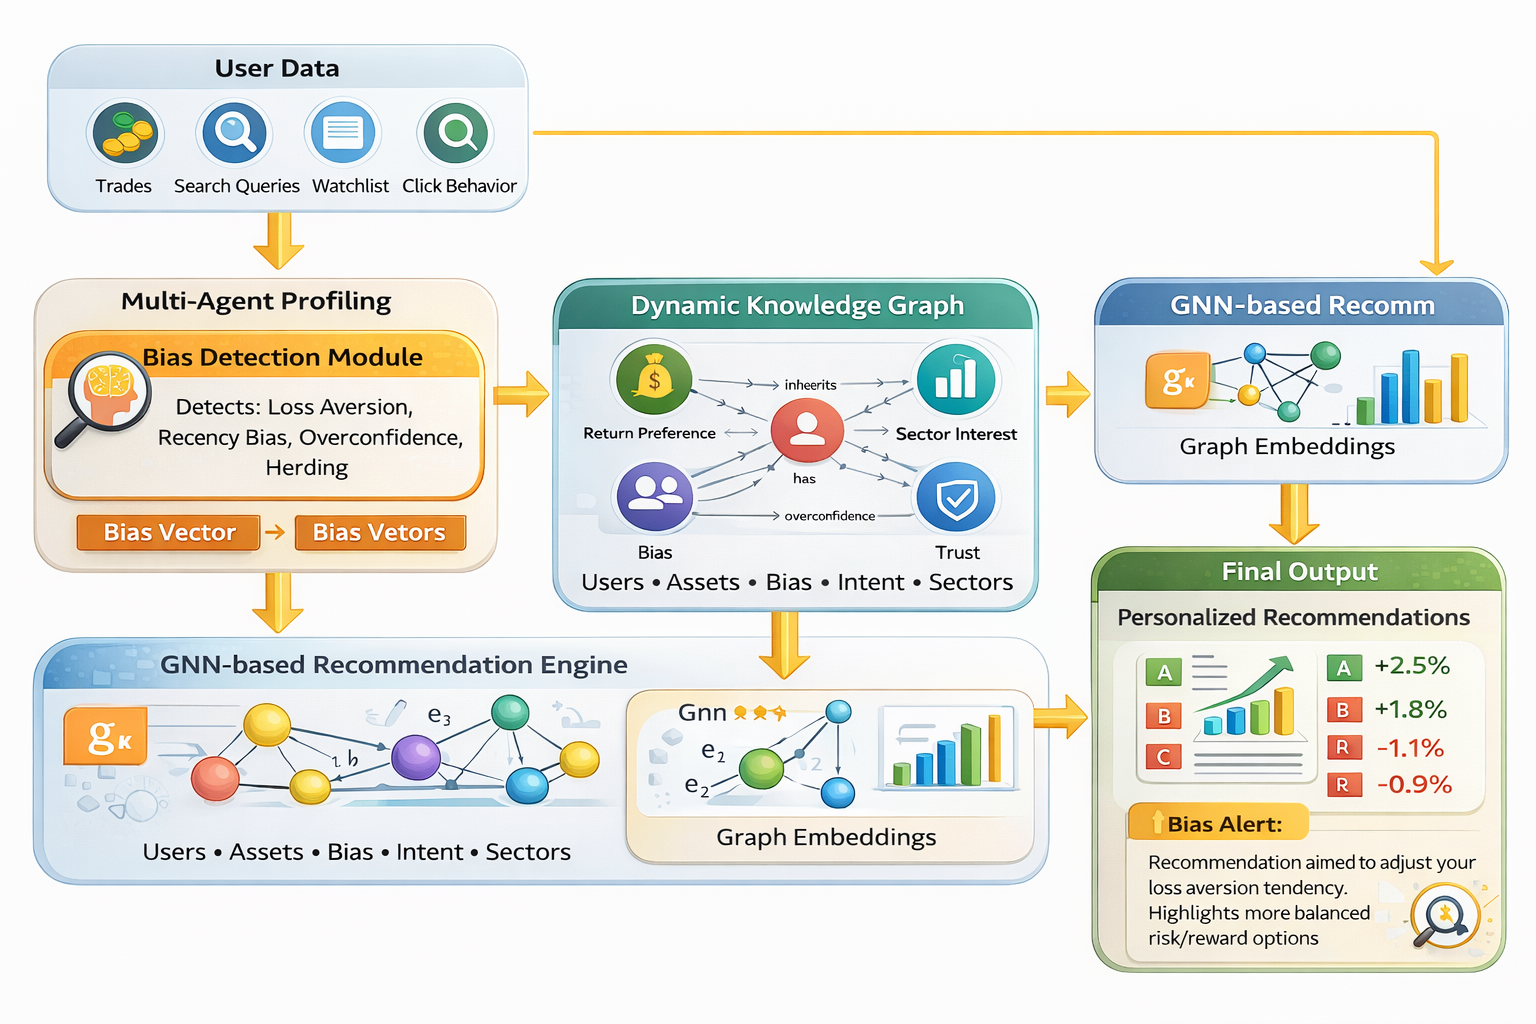
\includegraphics[width=0.95\textwidth]{figures/flow_chart.png}
\caption{FINDEC-RS Data Flow Diagram. Illustrates how multiple data sources (behavioral logs, 
market data, sentiment feeds, and explicit user inputs) flow through the system components, 
converge in the Knowledge Graph, and ultimately produce bias-corrected recommendations and 
explanations for end users.}
\label{fig:data_flow}
\end{figure}

\subsubsection{Implementation Stack}

\begin{table}[H]
\centering
\caption{Technology Stack}
\renewcommand{\arraystretch}{1.4}
\begin{tabularx}{\textwidth}{>{\bfseries}lllX}
\toprule
\textbf{Layer} & \textbf{Technology} & \textbf{Version} & \textbf{Role} \\
\midrule
Frontend   & Next.js + TypeScript & 14      & Dashboard, recommendation feed, bias report UI \\
Backend    & FastAPI (Python)     & 3.11    & REST API, agent orchestration, JWT auth \\
KG Store   & Neo4j                & 5.x     & Dynamic Knowledge Graph persistence \\
GNN Model  & PyTorch Geometric    & 2.x     & GraphSAGE / GAT-based recommendation \\
ML Models  & scikit-learn + LSTM  & ---     & Bias classifier, intent modeler \\
Agents     & LangChain            & 0.3+    & Multi-agent pipeline orchestration \\
Market Data& yfinance, Alpha Vantage & ---  & Live asset prices and fund metadata \\
Auth       & JWT + Refresh Tokens & ---     & Secure user session management \\
Container  & Docker Compose       & ---     & Full-stack service orchestration \\
\bottomrule
\end{tabularx}
\end{table}

% ============================================================
\section{Evaluation Plan}

The system will be validated across four dimensions. A synthetic behavioural dataset will
simulate users with known bias profiles for ground-truth evaluation. A held-out test
split will be used for RS metric evaluation. Financial performance will be assessed via
paper-trading simulation over a 30-day horizon.

\begin{table}[H]
\centering
\caption{Evaluation Metrics}
\renewcommand{\arraystretch}{1.4}
\begin{tabularx}{\textwidth}{>{\bfseries}llX}
\toprule
\textbf{Category} & \textbf{Metric} & \textbf{Purpose} \\
\midrule
RS Standard        & Precision@K, Recall@K & Ranking quality at top-K positions \\
RS Standard        & NDCG@K                & Graded relevance-based ranking evaluation \\
RS Standard        & F1-Score              & Harmonic mean of precision and recall \\
RS Standard        & Novelty               & Proportion of non-obvious long-tail assets recommended \\
RS Standard        & Diversity             & Intra-list diversity of recommended asset types \\
Bias Correction    & Bias Reduction Score  & Pre- vs post-recommendation bias signal change \\
Financial          & Simulated Sharpe Ratio& Risk-adjusted return in paper-trading simulation \\
Explainability     & KG path coherence     & Logical validity of explanation chain \\
Classifier         & Accuracy              & Bias classification accuracy vs ground truth \\
\bottomrule
\end{tabularx}
\end{table}

% ============================================================
\section{Demonstration Plan}

At the end-of-semester demonstration, the group will present a live walkthrough of the
deployed web application covering:

\begin{itemize}[leftmargin=1.5cm]
  \item User onboarding flow with intent preference collection
  \item Live asset query submission (e.g., ``Suggest mid-cap funds in renewable energy under moderate risk'')
  \item Real-time bias detection result displayed on the dashboard
  \item Ranked recommendation output with KG-traced explanation chips
  \item Side-by-side comparison of recommendations before and after bias correction
  \item Evaluation metric dashboard showing Precision@K, NDCG, Novelty, and Diversity
  \item Bias profile evolution chart across simulated sessions
\end{itemize}

% ============================================================
\section{GUI / Web Interface}

The platform is built as a responsive web application with the following key views:

\begin{itemize}[leftmargin=1.5cm]
  \item \textbf{Dashboard:} Portfolio overview, bias profile radar chart, intent vector
        visualisation, session activity feed
  \item \textbf{Query Interface:} Natural-language or structured asset query input with
        filter controls (sector, risk, return target, fund manager)
  \item \textbf{Recommendation Feed:} Ranked cards with explanation chips, bias-correction
        badges (e.g., \textit{``Reduces recency bias''}), and intent-alignment scores
  \item \textbf{Bias Report:} Time-series view of bias dimension evolution across sessions
  \item \textbf{KG Explorer:} Interactive graph panel tracing the reasoning path from
        user node to recommended asset node
  \item \textbf{Portfolio Manager:} View and manage current holdings with bias-aware alerts
  \item \textbf{Settings:} User preference configuration and bias detection sensitivity tuning
\end{itemize}

% ============================================================
\section{Project Scope and Implementation Details}

\subsection{Project Scope}

FINDEC-RS focuses on equity and mutual fund recommendation for retail investors.
The midterm phase targets Indian retail investors as the primary cohort using
SEBI-registered fund data and NSE-listed equities as the asset universe. Derivatives,
commodities, and cryptocurrency are explicitly out of scope for this phase.

\subsection{Major Supported Operations}

\begin{enumerate}[leftmargin=1.5cm]
  \item User registration and bias-profile onboarding
  \item Intent vector construction from explicit preferences and implicit signals
  \item Dynamic Knowledge Graph construction and session-level update
  \item GNN-based personalised asset ranking with bias correction
  \item Natural-language explanation generation per recommendation
  \item Report history storage and retrieval via authenticated API
  \item Evaluation dashboard with live metric computation
  \item Admin panel for dataset management and model retraining
\end{enumerate}

% ============================================================
\newpage
\addcontentsline{toc}{section}{References}

\section*{References}

\begin{thebibliography}{99}

\bibitem{biases2025}
H. K. Baker, G. Filbeck, and V. Ricciardi,
\textit{Biases in Behavioral Finance},
World Scholars Review, vol. 3, no. 1, pp. 1--18, 2025.

\bibitem{robo2025}
M. Cemri, M. Z. Pan, S. Yang, et al.,
\textit{Cognitive Biases, Robo Advisor and Investment Decision Psychology},
ScienceDirect (Elsevier), 2025.
\url{https://doi.org/10.1016/j.joep.2025.102788}

\bibitem{debias_survey}
J. Chen, H. Dong, X. Wang, F. Feng, M. Wang, and X. He,
\textit{Bias and Debias in Recommender System: A Survey and Future Directions},
ACM Transactions on Information Systems, vol. 41, no. 3, pp. 1--39, 2023.
\url{https://doi.org/10.1145/3564284}

\bibitem{stanford_intent2025}
S. Wang, C. Banerjee, S. Chucri, and M. Chen,
\textit{IS-Rec: Intent-Structured Whole-Page Recommender System},
Stanford HAI / Google DeepMind, 2025.

\bibitem{popularity_bias2025}
M. Deldjoo, T. Di Noia, and B. Schedl,
\textit{Popularity Bias in Recommender Systems: The Search for Fairness in the Long Tail},
Information, vol. 16, no. 2, p. 151, Feb. 2025.
\url{https://doi.org/10.3390/info16020151}

\bibitem{fund_kg2023}
H. Li, J. Du, G. Liu, F. Jiang, Y. Wang, and X. Zhou,
\textit{Disentangled Interest Importance Aware Knowledge Graph Neural Network for
Fund Recommendation},
Proc. 32nd ACM CIKM, 2023.
\url{https://doi.org/10.1145/3583780.3614846}

\bibitem{gnn_survey_tors}
C. Gao, Y. Zheng, N. Li, Y. Li, Y. Qin, J. Piao, Y. Quan, J. Chang, D. Jin,
X. He, and Y. Li,
\textit{A Survey of Graph Neural Networks for Recommender Systems: Challenges,
Methods, and Directions},
ACM Transactions on Recommender Systems, vol. 1, no. 1, 2023.
\url{https://doi.org/10.1145/3568022}

\bibitem{lightgnn2025}
X. Chen, C. Huang, Y. Zhang, and H. Yin,
\textit{LightGNN: Simple Graph Neural Network for Recommendation},
Proc. 18th ACM WSDM, pp. 1--10, Mar. 2025.
\url{https://arxiv.org/abs/2501.03228}

\bibitem{gnn_topo2025}
D. Malitesta, C. Pomo, F. Merra, T. Di Noia, and E. Di Sciascio,
\textit{On the Impact of Graph Neural Networks in Recommender Systems:
A Topological Perspective},
arXiv preprint arXiv:2512.07384, Dec. 2025.
\url{https://arxiv.org/abs/2512.07384}

\bibitem{rdf_gnn2025}
D. Malitesta, G. Cornacchia, C. Pomo, F. Merra, T. Di Noia, and E. Di Sciascio,
\textit{Bridging RDF Knowledge Graphs with Graph Neural Networks for
Semantically-Rich Recommender Systems},
arXiv preprint arXiv:2506.08743, Jun. 2025.
\url{https://arxiv.org/abs/2506.08743}

\bibitem{kgrs_survey}
Y. Guo, X. Zhao, and C. Shi,
\textit{Deep Learning on Knowledge Graph for Recommender System: A Survey},
arXiv preprint arXiv:2004.00387, 2020.
\url{https://arxiv.org/abs/2004.00387}

\bibitem{multiagent_recsys2025}
V. W. Anelli, Y. Deldjoo, T. Di Noia, A. Ferrara, and F. Narducci,
\textit{Multi-Agentic Recommender Systems: Foundations, Design Patterns, and
E-Commerce Applications},
Proc. 19th ACM RecSys (Tutorial), 2025.
\url{https://doi.org/10.1145/3705328.3748008}

\bibitem{agentic_rs2025}
X. Zhu, Y. Wang, H. Gao, W. Xu, et al.,
\textit{Recommender Systems Meet Large Language Model Agents: A Survey},
Foundations and Trends in Privacy and Security, vol. 7, no. 4, pp. 247--396, 2025.

\bibitem{llm_agents_finance2025}
G. Fatouros, K. Metaxas, J. Soldatos, and M. Karathanassis,
\textit{Large Language Model Agents for Investment Management: Foundations,
Benchmarks, and Research Frontiers},
Proc. 6th ACM International Conference on AI in Finance (ICAIF), 2025.
\url{https://doi.org/10.1145/3768292.3770387}

\bibitem{llm_mas_finance2025}
Q. Peng, H. Liu, H. Huang, J. Yang, Q. Yang, and M. Shao,
\textit{A Survey on LLM-powered Agents for Recommender Systems},
Proc. EMNLP Findings, Nov. 2025.
\url{https://aclanthology.org/2025.findings-emnlp.620}

\bibitem{heterollm2025}
Y. Xiao, E. Sun, D. Luo, and W. Wang,
\textit{Designing Heterogeneous LLM Agents for Financial Sentiment Analysis},
ACM Transactions on Management Information Systems, 2025.
\url{https://doi.org/10.1145/3688399}

\bibitem{intent_cf2025}
H. Li, J. Du, G. Liu, F. Jiang, Y. Wang, and X. Zhou,
\textit{Intent Propagation Contrastive Collaborative Filtering},
IEEE Transactions on Knowledge and Data Engineering, vol. 37, no. 5,
pp. 2665--2679, May 2025.
\url{https://doi.org/10.1109/TKDE.2025.3543241}

\end{thebibliography}

\end{document}
